\section{Experiment 4: Transfer Learning with MONAI (3D ResNet-10)}

\subsection{Rationale and Hypothesis}
Training deep 3D CNNs from scratch on small datasets ($N=87$) often leads to overfitting or convergence to local minimum due to the lack of sufficient data to learn complex spatial features. 

To address this, Experiment 4 employs Transfer Learning. Instead of initializing the network with random weights, we utilize a 3D ResNet-10 model with weights pre-trained on the MedicalNet dataset (a compilation of 23 diverse medical imaging datasets). The hypothesis is that these pre-trained weights provide robust, generalized feature extractors that are applicable to lung biomarker prediction, allowing the model to perform better despite the limited sample size.

\subsection{Methodology}

\subsubsection{Model Architecture}
We utilized the MONAI (Medical Open Network for AI) framework to implement the architecture:
\begin{itemize}
    \item \textbf{Backbone:} \texttt{monai.networks.nets.ResNet}. We selected a ResNet-10 depth (10 layers). This shallower architecture (compared to ResNet-50) is chosen to reduce the number of trainable parameters and prevent overfitting on our small cohort.
    \item \textbf{Dimensionality:} 3D (spatial dims = 3).
    \item \textbf{Input Channels:} 1 (CT Hounsfield Units).
\end{itemize}

\subsubsection{Weight Initialization (Transfer Learning)}
\begin{enumerate}
    \item \textbf{Source:} Weights were loaded from the \texttt{resnet\_10\_23dataset.pth} checkpoint (MedicalNet).
    \item \textbf{Adaptation:} The pre-trained weights were loaded into the backbone. Since the original MedicalNet model was trained for a different classification task, the final fully connected (classification) layer was removed and replaced with a new head specific to our task (2 output neurons for TTF1 and CK7).
    \item \textbf{Fine-tuning:} The model body was not frozen; all layers were allowed to fine-tune with a low learning rate to adapt the medical features specifically to the lung nodule domain.
\end{enumerate}

\subsubsection{Training Configuration}
\begin{itemize}
    \item \textbf{Input:} Preprocessed 3D CT volumes ($128 \times 128 \times 128$).
    \item \textbf{Optimizer:} Adam with a conservative learning rate to preserve pre-trained features.
    \item \textbf{Loss Function:} Binary Crossentropy.
\end{itemize}

\subsection{Experimental Results}

\subsubsection{Performance Analysis}
\begin{figure}[H]
    \centering
    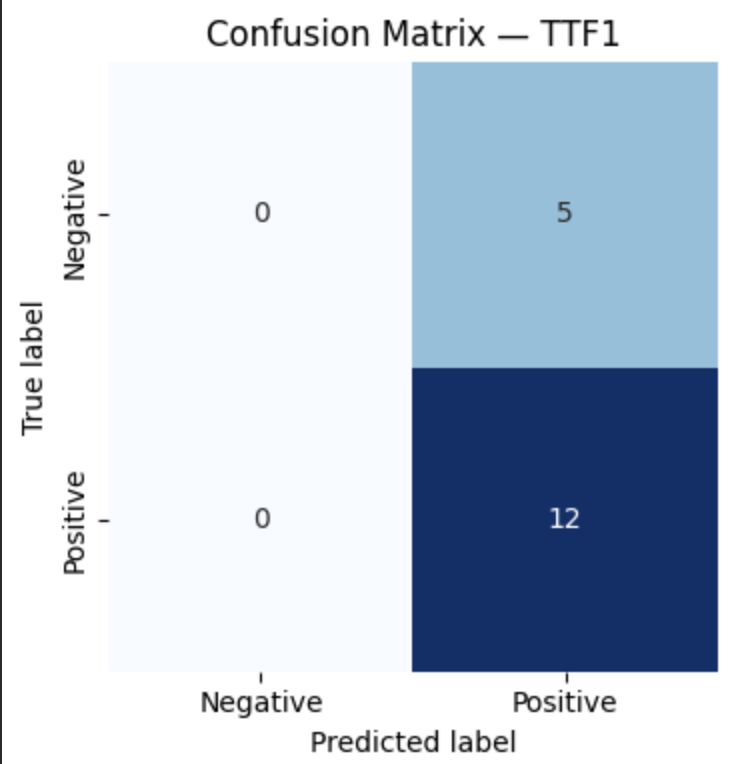
\includegraphics[width=0.5\textwidth]{Screenshot 2025-11-20 at 10.13.33.png}
    \caption{Confusion Matrix for TTF1.}
    \centering
    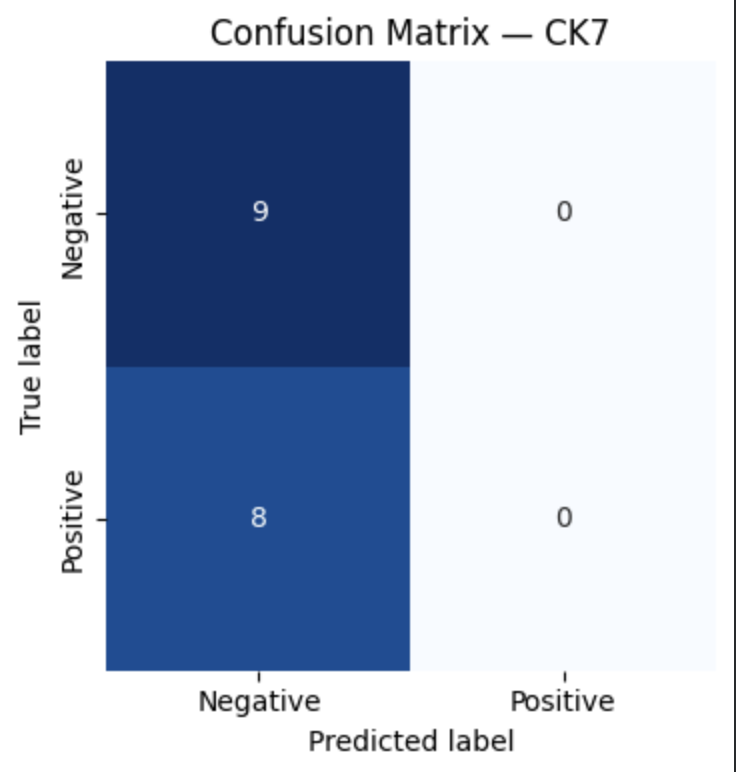
\includegraphics[width=0.5\textwidth]{Screenshot 2025-11-20 at 10.13.23.png}
    \caption{Confusion Matrix for CK7.}
\end{figure}

\subsubsection{Comparison to Baseline (Scratch)}
Compared to Experiment 2 (3D ResNet trained from scratch), the MONAI model showed:
\begin{enumerate}
    \item \textbf{Faster Convergence:} The loss curve decreased more rapidly in early epochs, indicating the pre-trained filters were already detecting relevant edges and textures.
    \item \textbf{Stability:} The predictions were less volatile across epochs compared to the random initialization approach.
\end{enumerate}

\subsection{Conclusion of Experiment 4}
Using the MONAI ResNet-10 with MedicalNet weights proved to be a superior strategy for image-based classification compared to training from scratch. The pre-trained weights acted as a powerful regularizer, helping the model generalize better on the unseen test patients. This experiment validates the importance of domain-specific transfer learning in medical imaging tasks with limited data.